\chapter{Proposed Methodology}
\label{chap:methodology}

In our proposed methodology, we aim to leverage the strengths of both the UniCL framework and the Swin Transformer architecture to enhance the performance of our model. The methodology is structured into several key components, each addressing a specific aspect of the overall process. The following sections provide a detailed overview of each component, including the backbone architecture, CAM generation, pseudo label generation, segmentation prediction, and refinement.


\section{Background}
\label{sec:background}

In this section, we will discuss the background of the proposed methodology, including the concepts of Class Activation Maps (CAMs), the backbone architecture, and the process of generating pseudo labels. We will also provide an overview of the UniCL framework and its components, as well as the Swin Transformer architecture and its advantages for image segmentation tasks

\subsection{Multi-Modal Learning}
\label{subsec:multi_modal_learning}
Multi-modal learning refers to the process of learning from multiple sources of information, such as images and text. This approach allows models to leverage complementary information from different modalities, leading to improved performance on various tasks. For example, in classification tasks, the ability to learn from both images and text enables the model to capture richer semantic information, enhancing its understanding of the data. More importantly, it can enable zero-shot capabilities, where the model can classify images it has never seen before. This is achieved by associating the visual features of an image with its textual description, allowing the model to generalize to unseen classes. As classification is often a foundational step in many processes, this ability is highly valuable.

\subsubsection{Contrastive Learning}
\label{subsec:contrastive_learning}
Contrastive learning is a self-supervised learning approach that aims to learn representations by contrasting positive and negative pairs. This involves aligning features from related inputs (e.g., an image and its corresponding text description) in a shared embedding space while ensuring that unrelated features are pushed apart. A contrastive loss function is typically used to minimize the distance between positive pairs while maximizing the distance between negative pairs. This approach helps models learn discriminative and meaningful representations that are robust and generalizable.

\subsubsection{Training Strategy}
\label{subsec:training_strategy}
The training strategy for multi-modal learning often involves a combination of supervised and self-supervised learning techniques. Models are trained on large-scale datasets containing paired samples from different modalities, enabling them to learn meaningful representations through techniques like contrastive learning. Data augmentation is frequently employed to improve the robustness and diversity of the learned features, ensuring better generalization to unseen data.

\subsubsection{Task-Agnostic Learning}
\label{subsec:task_agnostic_learning}
Task-agnostic learning refers to the ability of a model to learn representations that are not specifically tailored to a single task but can be applied across various tasks. This is achieved by focusing on learning generalizable features that are beneficial for multiple downstream applications. By training on diverse datasets and leveraging multi-modal information, models can develop representations that are adaptable to different tasks, such as image classification, object detection, and image segmentation. This flexibility makes task-agnostic learning a powerful approach for building versatile and reusable models.

\subsection{Contrastive Language-Image Pre-Training (CLIP)}
\label{subsec:clip}

CLIP \cite{vl_clip} is a multi-modal learning framework that leverages contrastive learning to align images and text in a shared embedding space. It is designed to learn representations that can generalize across various tasks without requiring task-specific fine-tuning. CLIP achieves this by training on a large dataset of image-text pairs, allowing it to learn meaningful relationships between visual and textual information.

\subsection{CLIP Architecture}
\label{subsec:clip_architecture}

\subsubsection{CLIP Components}
CLIP consists of two main components:

\begin{itemize}
    \item \textbf{Image Encoder}: This component is responsible for processing images and extracting features. It typically includes a swin transformer, pooling layers, and other modules designed to capture spatial hierarchies and relationships within the image data.
    \item \textbf{Text Encoder}: This component processes text data, converting it into a format suitable for comparison with image features. It often includes transformer layers and attention mechanisms to capture the semantic relationships within the text.
\end{itemize}

The learning of CLIP is achieved through a contrastive loss function that aligns the image and text features in a shared embedding space. This allows the model to learn meaningful representations that can be applied to various tasks, such as image classification, object detection, and image segmentation. Or, in our case, weakly supervised semantic segmentation, which requires only image-level classification.

\subsection{Unified Contrastive Learning (UniCL)}
\label{subsec:unicl}

UniCL, short for Unified Contrastive Learning \cite{vl_unicl}, is another multi-modal learning framework that builds upon the principles of CLIP. It aims to unify various contrastive learning approaches into a single framework, allowing for more efficient and effective learning from multiple modalities.

But it is not just a simple extension of CLIP. UniCL introduces several key innovations that enhance its performance and versatility.

First, UniCL employs a unified architecture that combines image-label and text-label contrastive learning into a single framework, making a image-label-text space. This allows the contrastive learning process to be more efficient and effective. Because, in the image-text space, in contrastive learning, the model learns to increase the similarity between the image and text features while decreasing the similarity between unrelated features. CLIP used to assume the image-text pair, that was provided as input, to be the only positive pair. But in reality, there are many other positive pairs in the dataset. For example, if we have an image of a cat and the text "a photo of a cat" is provided as input, then another similar text, "a photo of a kitten" can also be a positive pair. CLIP does not consider this. but UniCL does. It tries to learn the similarity between the image and all the text features that have the same category as the image. This is done by using a contrastive loss function that encourages the model to learn a shared representation space for both images and text.

\subsubsection{Unified Image-Text-Label Contrast in UniCL}
\label{subsec:unified_image_text_label_contrast}

UniCL employs a bidirectional learning objective between image-text pairs:
\begin{equation} \label{eq:unified_image_text_label_contrast}
    \min_{\{\theta, \phi\}} \mathcal{L}_{\text{BiC}} = \mathcal{L}_{i2t} + \mathcal{L}_{t2i},
\end{equation}
where \(\mathcal{L}_{i2t}\) and \(\mathcal{L}_{t2i}\) are the image-to-text and text-to-image contrastive losses, respectively. And \(\theta\) and \(\phi\) are the parameters of the image and text encoders, respectively.

The image-to-text contrastive loss to align matched images in a batch with a given text is defined as:
\begin{equation} \label{eq:unicl_image_to_text_contrastive_loss}
    \mathcal{L}_{i2t} = - \sum_{i \in \mathcal{B}} \frac{1}{|\mathcal{P}(i)|} \sum_{k \in \mathcal{P}(i)} 
    \log \frac{\exp(\tau \mathbf{u}_i^\top \mathbf{v}_k)}{\sum_{j \in \mathcal{B}} \exp(\tau \mathbf{u}_i^\top \mathbf{v}_j)},
\end{equation}
where $k \in \mathcal{P}(i) = \{k | k \in \mathcal{B}, y_k = y_i\}$, i.e., the set of all images in the batch that belong to the same class as image $i$.

On the other hand, the text-to-image contrastive loss to align matched text in a batch with a given image is defined as:

\begin{equation} \label{eq:unicl_text_to_image_contrastive_loss}
    \mathcal{L}_{t2i} = - \sum_{j \in \mathcal{B}} \frac{1}{|\mathcal{P}(j)|} \sum_{k \in \mathcal{P}(j)} 
    \log \frac{\exp(\tau \mathbf{u}_k^\top \mathbf{v}_j)}{\sum_{i \in \mathcal{B}} \exp(\tau \mathbf{u}_i^\top \mathbf{v}_j)},
\end{equation}
where $k \in \mathcal{P}(j) = \{k \mid k \in \mathcal{B}, y_k = y_j\}$, i.e., the set of all text features in the batch that belong to the same class as text $j$.

\subsubsection{Comparison with CLIP}
\label{subsec:clip_vs_unicl}

In case CLIP, for an image, there is only one positive text feature. In other words, $\mathcal{P}(i) = {i} \in \mathcal{B}$; and $\mathcal{P}(j) = {j} \in \mathcal{B}$. So, the image-to-text contrastive loss is defined as:

\begin{equation} \label{eq:clip_image_to_text_contrastive_loss}
    \mathcal{L}_{i2t} = - \sum_{i \in \mathcal{B}} 
    \log \frac{\exp(\tau \mathbf{u}_i^\top \mathbf{v}_i)}{\sum_{j \in \mathcal{B}} \exp(\tau \mathbf{u}_i^\top \mathbf{v}_j)},
\end{equation}
where $i \in \mathcal{B}$ is the index of the image in the batch.

And the text-to-image contrastive loss is defined as:

\begin{equation} \label{eq:clip_text_to_image_contrastive_loss}
    \mathcal{L}_{t2i} = - \sum_{j \in \mathcal{B}} 
    \log \frac{\exp(\tau \mathbf{u}_j^\top \mathbf{v}_j)}{\sum_{i \in \mathcal{B}} \exp(\tau \mathbf{u}_i^\top \mathbf{v}_j)},
\end{equation}
where $j \in \mathcal{B}$ is the index of the text feature in the batch. 

The equations \ref{eq:unified_image_text_label_contrast}-\ref{eq:clip_text_to_image_contrastive_loss} are taken from \cite{vl_unicl}.

This means that $\mathcal{L}_{BiC}$ becomes CLIP training objective. The main property in \autoref{eq:unicl_text_to_image_contrastive_loss} is that for each image feature, any of the text features in the batch can be used as a positive pair. And so is the case for \autoref{eq:unicl_text_to_image_contrastive_loss}.

Second, UniCL replaces CLIP's ViT backbone with a Swin Transformer backbone. The Swin Transformer is a hierarchical vision transformer that captures both local and global information in images, making it more suitable for various vision tasks.

\subsection{Swin Transformer}
\label{subsec:swin_transformer}
Swin Transformer is a hierarchical vision transformer that employs a shifted windowing scheme to capture both local and global information in images. It is designed to be computationally efficient while maintaining high performance on various vision tasks. The architecture consists of multiple stages, each with its own set of transformer blocks, allowing it to process images at different resolutions and capture multi-scale features.

\autoref{fig:swin_vs_vit_architecture} illustrates the architectures of the Swin Transformer and Vision Transformers (ViT). The key distinction lies in their processing strategies: the Swin Transformer employs a hierarchical structure, processing feature maps at multiple resolutions, while ViT processes the entire image globally at a single resolution. This hierarchical approach enables the Swin Transformer to effectively capture both local and global information, making it particularly suitable for tasks requiring fine-grained details alongside overall context.

The Swin Transformer builds hierarchical feature maps by progressively merging image patches (depicted in gray) in deeper layers. It computes self-attention only within local windows (highlighted in red), resulting in linear computational complexity relative to the input image size. This efficiency, combined with its ability to handle dense recognition tasks, makes it a versatile backbone for both image classification and segmentation.

In contrast, traditional vision Transformers, such as ViT, produce feature maps at a single low resolution and compute self-attention globally, leading to quadratic computational complexity with respect to the input image size. This global attention mechanism, while effective for certain tasks, is less efficient for dense prediction tasks compared to the Swin Transformer's localized attention mechanism.

\begin{figure}[htbp]
    \centering
    \fbox{ % Draw a box around the entire figure
        \begin{minipage}{0.9\textwidth} % Adjust the width as needed
            \begin{subfigure}[b]{0.45\textwidth}
                \centering
                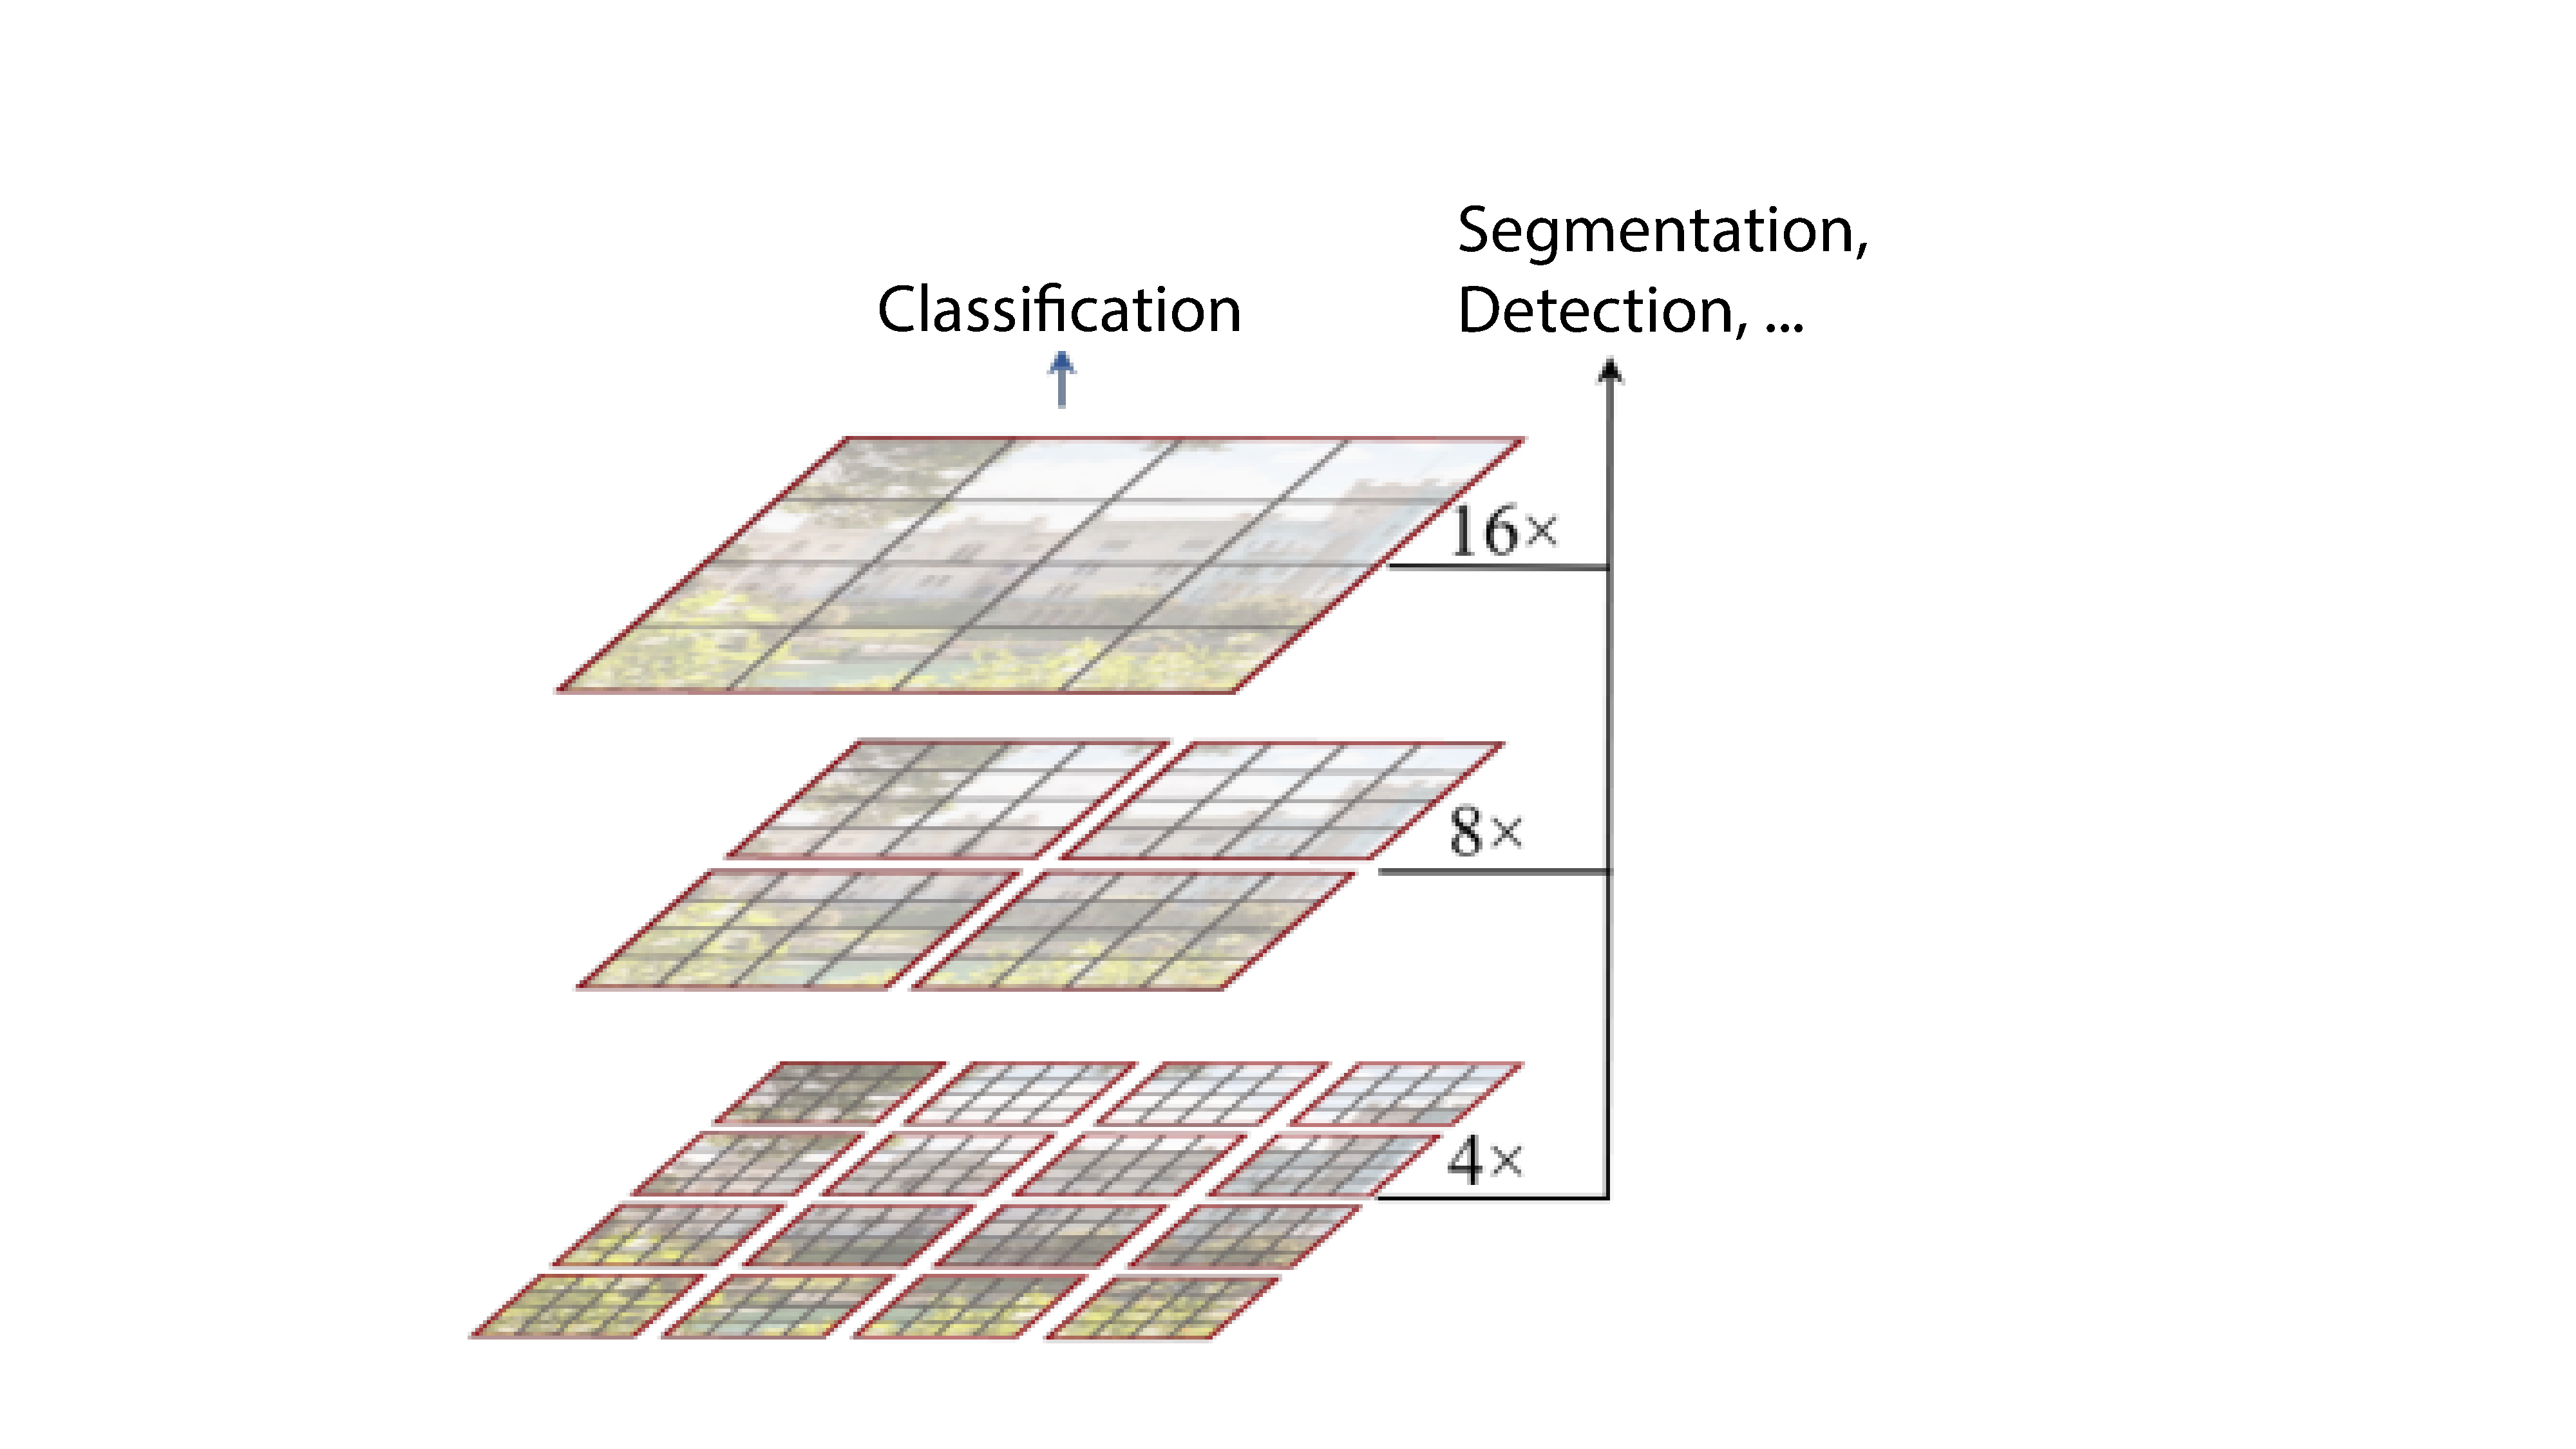
\includegraphics[width=\textwidth]{swin-vs-vit-archi-a.pdf}
                \caption{Swin Transformer}
                \label{fig:swin_transformer_data_flow}
            \end{subfigure}
            \hfill
            \begin{subfigure}[b]{0.45\textwidth}
                \centering
                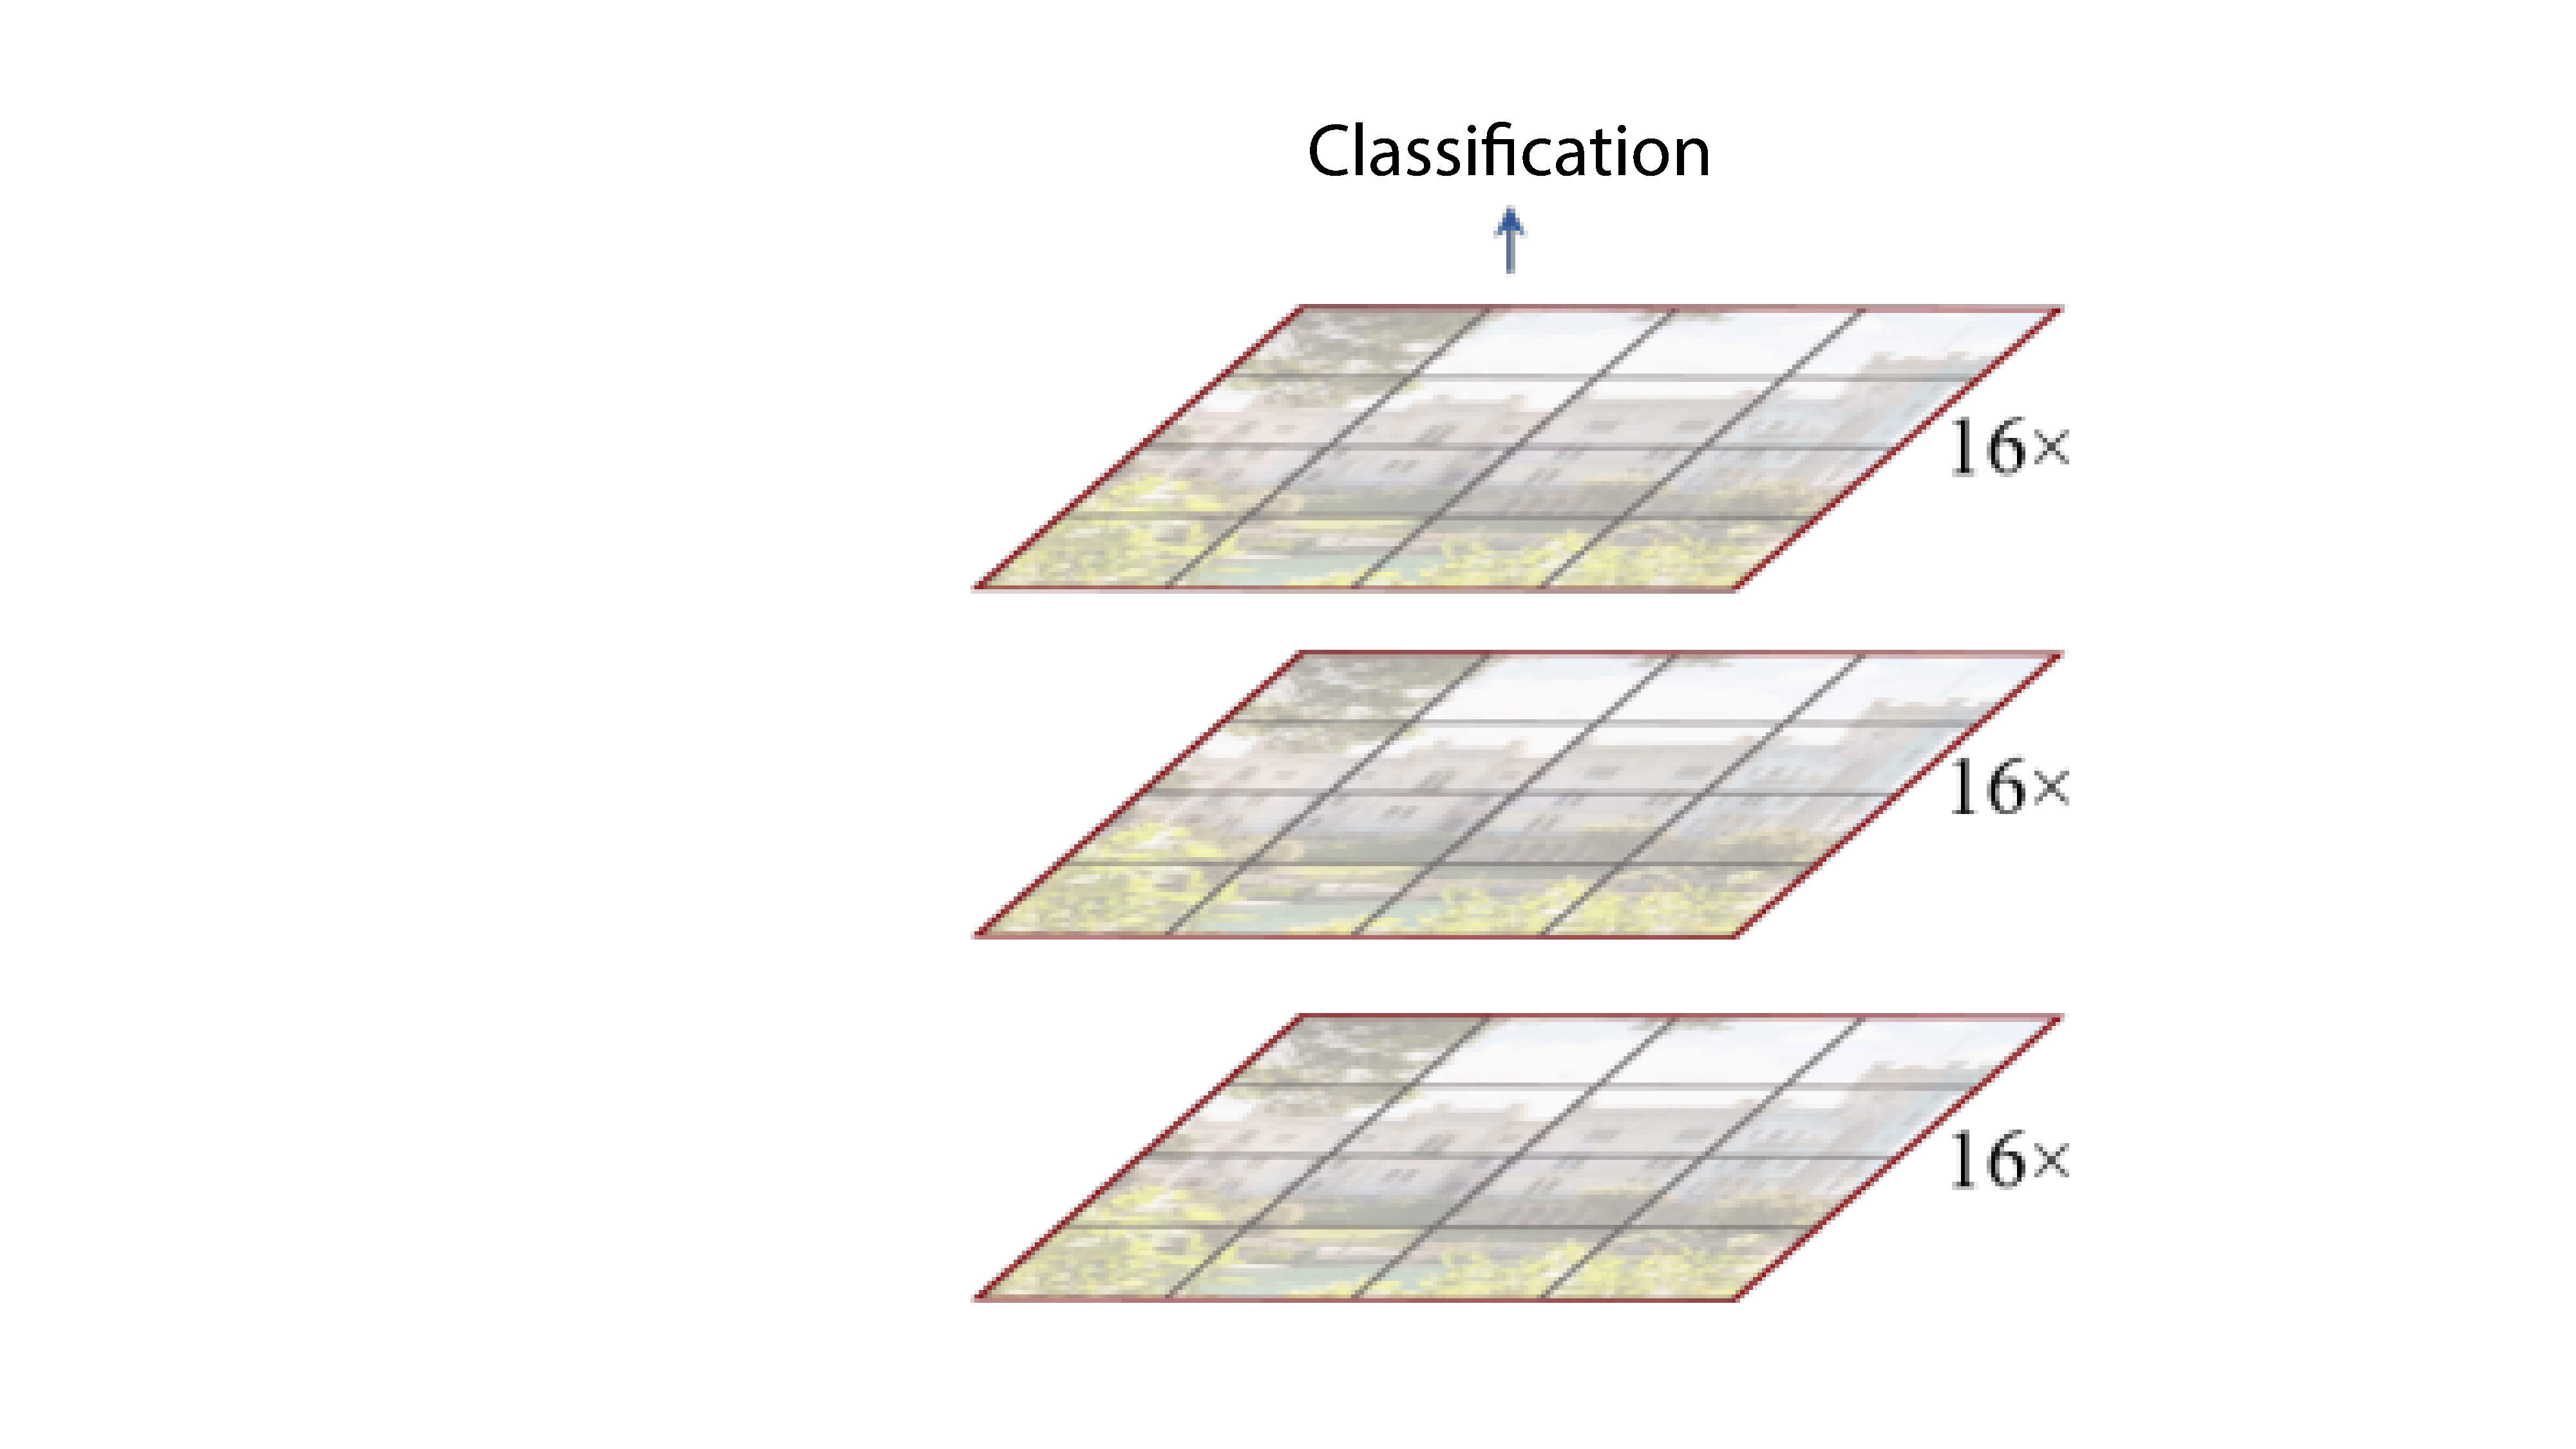
\includegraphics[width=\textwidth]{swin-vs-vit-archi-b.pdf}
                \caption{Vision Transformers}
                \label{fig:vit_data_flow}
            \end{subfigure}
        \end{minipage}
    }
    \caption{Comparison of Swin Transformer and ViT Architectures}
    \label{fig:swin_vs_vit_architecture}
\end{figure}

Because of the hierarchical nature of the Swin Transformer, it is particularly well-suited for tasks that require a combination of global context (to indentify the overall structure of the image) and local details (to capture fine-grained features, e.g., edges, textures). This makes it a strong candidate for image segmentation tasks.

Also, the Contrastive and Multi-Modal Learning capabilities of UniCL can be effectively combined with the Swin Transformer's hierarchical architecture to enhance the model's ability to learn rich and discriminative features from both image and text modalities. This combination allows for a more comprehensive understanding of the data, leading to improved performance.

Now, getting all the background information, we can proceed to the proposed methodology. The proposed methodology consists of several key components, including the backbone architecture, CAM generation, pseudo label generation, segmentation prediction, and refinement. Each component plays a crucial role in enhancing the overall performance of the model.

\begin{figure}
    \centering
    \fbox{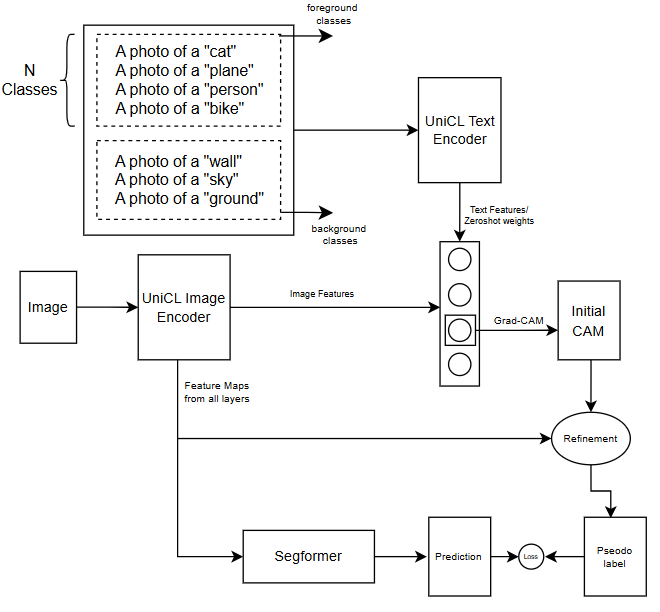
\includegraphics[width=0.9\textwidth]{architecture.png}}
    \caption{architecture}
    \label{fig:architecture}
\end{figure}

\section{Backbone}
\label{sec:backbone}

As we have seen so far, the pseudo labels and CAMs are two critical components of WSSS. First of all, the CAMs are generated from the backbone network, using which the pseudo labels are generated. The pseudo labels are then used to train the segmentation head (or segmentation model in case of multi-stage approach).

So the more accurate the initial CAMs are, the better the pseudo labels will be. And so will be the segmentation model. So we need to ensure that the CAMs are as accurate as possible. Keeping this in mind, we are experimenting with different backbone architectures to find the one that generates the most accurate CAMs.

So, we have chosen UniCL as the first one to experiment with. The reason is that it is a multi-modal model, and it has been shown to produce high-quality CAMs. It is also a state-of-the-art model for zero-shot image classification. So, we can expect it to produce high-quality CAMs.

\section{CAM Generation}
\label{sec:cam_generation}

\autoref{fig:cam_generation_process_clip} shows the process of generating CAMs using CLIP/UniCL. We have used Grad-CAM. The process is similar to the method discussed in \autoref{subsec:grad_cam}, which is used to generate CAMs using CNN-based models.
 But there are some differences.

AS CLIP is a multi-modal model, the main classification task is to find similarity between the image and text.

If we want to generate the CAM for $N$ classes, we need to provide $N$ text features as input. So, at the very beginning, we need to encode the text features using the CLIP text encoder, and store them.

An MLP layer basically takes the linear combination of the input features and the weights. We do the same thing when finding similarity score between the image and text features, take the linear combination of the image features and the text features. So, we can consider these text features as the "neuron weights" of the classifier head.

Then, we need to pass the image through the CLIP image encoder to get the feature maps. The rest of the process is the same as Grad-CAM.


\begin{figure}[htbp]
    \centering
    \fbox{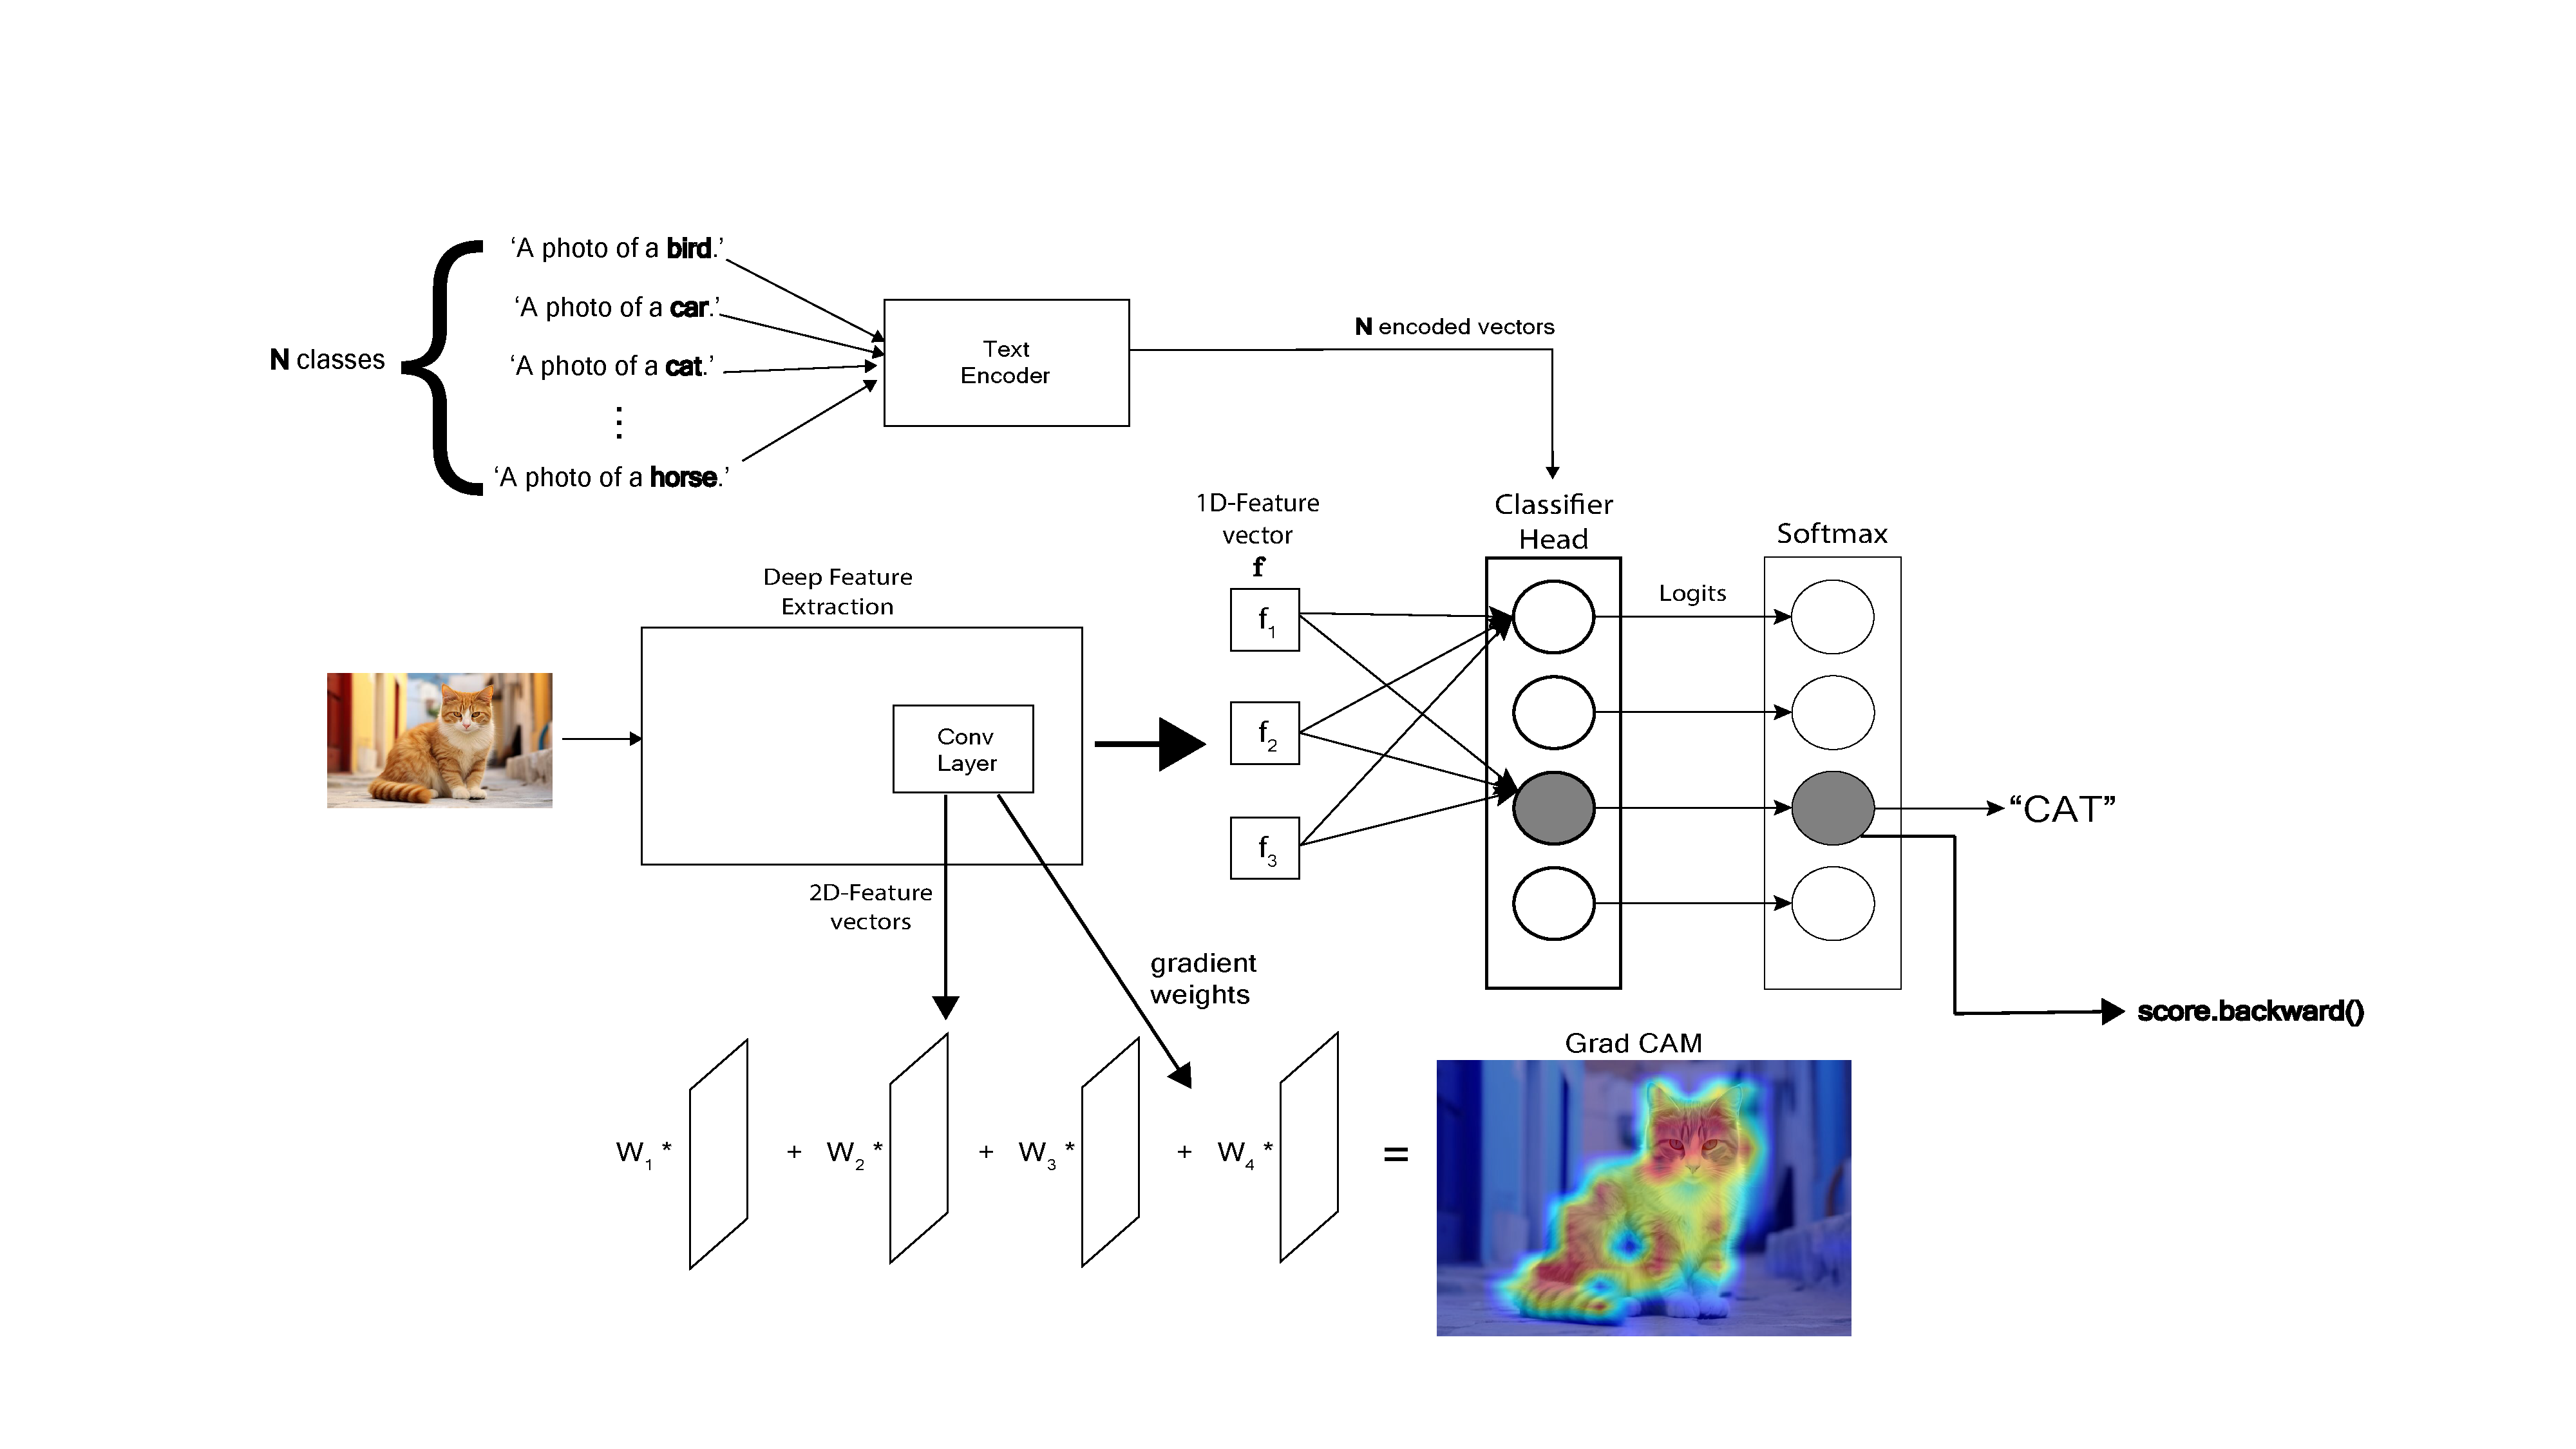
\includegraphics[width=0.8\textwidth]{clip-grad-cam.pdf}}
    \caption{CAM Generation Process using CLIP}
    \label{fig:cam_generation_process_clip}
\end{figure}

\section{Segmentation Prediction}
\label{sec:segmentation_prediction}
The segmentation prediction module is designed to generate pixel-wise class predictions for the input image. It consists of two main components: encoder feature aggregation and a decoder with multi-head transformer layers. It is constructed following \cite{wsss_frozen_clip}.

\subsection{Encoder Feature Aggregation}
\label{subsec:en_feature_agg}
Following \cite{wsss_frozen_clip}, the feature maps from the transformer blocks of the UniCL \cite{vl_unicl} image encoder need to be passed to the decoder. Let the feature maps be \( F_l^{\text{init}} \) for \( l = 1, \dots, N \) from the output of each transformer block in the encoder, where \( l \) represents the index of the block. Then, for each feature map \( F_l^{\text{init}} \), an individual MLP module is used to generate new corresponding feature maps \( F_l^{\text{new}} \):
\begin{equation}
    F_l^{\text{new}} = W_{1}^{\text{fc}} \left( \text{ReLU} \left( W_{2}^{\text{fc}}(F_l^{\text{init}}) \right) \right),
\end{equation}
where \( W_{1}^{\text{fc}} \) and \( W_{2}^{\text{fc}} \) are two different fully-connected layers, and \(\text{ReLU}(\cdot)\) is the ReLU activation function.


After that, all new feature maps \( F_l^{\text{new}} \) for \( l = 1, \dots, N \) are concatenated together, which are then processed by a convolution layer to generate a fused feature map \( F_u \):
\begin{equation}
    F_u = \text{Conv}\left( \text{Concat}\left[ F_1^{\text{new}}, F_2^{\text{new}}, \dots, F_N^{\text{new}} \right] \right),
    \tag{2}
\end{equation}

where \( F_u \in \mathbb{R}^{d \times h \times w} \), and \( d \), \( h \), and \( w \) represent the channel dimension, height, and width of the feature map, respectively. \(\text{Conv}(\cdot)\) is a convolutional layer, and \(\text{Concat}[\cdot]\) denotes the concatenation operation.


\begin{figure}[t]
    \centering
    \fbox{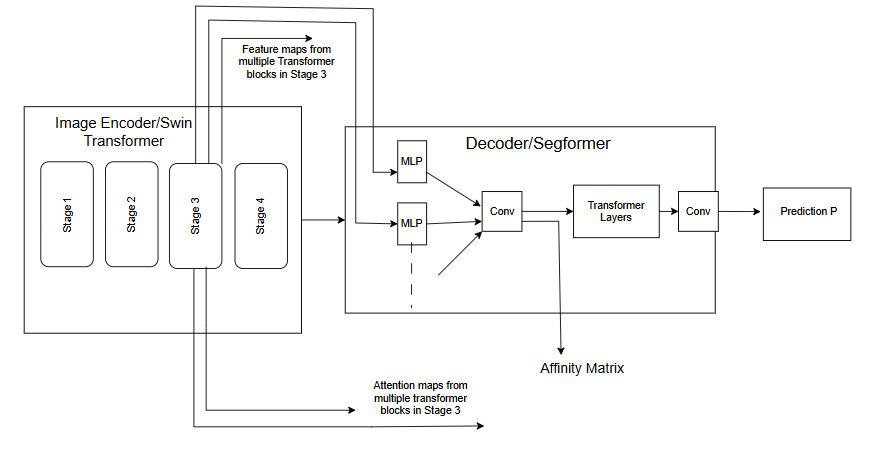
\includegraphics[width=0.9\textwidth]{decoder.png}}
    \caption{Decoder architecture}
    \label{fig:decoder}
\end{figure}

\subsection{Generating Final Prediction}
\label{subsec:decoder_final_pred}

Several sequential multi-head transformer layers are designed to generate the final prediction \( P \):
\begin{equation}
    \label{eq:prediction}
    P = \text{Conv}(\phi(F_u)) \uparrow,
\end{equation}
where \( P \in \mathbb{R}^{C \times H \times W} \), \( C \) is the number of classes including background, and \(\phi\) represents the sequential multi-head transformer blocks [12]. Each transformer block contains a multi-head self-attention module, a feed-forward network, and two normalization layers. The operator \(\uparrow\) denotes an upsampling operation to align the prediction map size with the original image.


\section{CAM Refinement and Pseudo-Label Generation}
\label{sec:refinement}
\subsection{Affinity based CAM refinement}  
The initial CAMs produced by the backbone tend to focus only on sparse, highly discriminative regions. These activations are often noisy and insufficient to be used directly as supervision. Therefore, a refinement module is required where the initial CAM is improved. The refined CAM is then used as a pseudolabel for supervision.  

The most common strategy for rectifying CAMs is by exploiting the feature relationships within the backbone that generates them. This is referred to as affinity-based CAM refinement, first introduced by \cite{wsss_affinitynet}. In transformer-based backbones, the attention maps naturally encode semantic-level affinities between tokens or patches. From these attention maps, an affinity matrix $A_f$ can be constructed and employed for CAM refinement via random walk propagation. In parallel, another affinity matrix, $\hat{A}$, can be derived from the predicted pseudolabel produced by the decoder. The cross-entropy loss between these two affinity matrices is then incorporated into the training objective.  

However, in our case, the backbone responsible for generating the CAMs is \textbf{frozen}, meaning that its attention maps remain fixed and do not update during training. To address this limitation, Frozen CLIP \cite{wsss_frozen_clip} proposes utilizing the affinity derived from intermediate features of the encoder instead of directly relying on the backbone’s frozen attention. The backbone attention maps are then used only to influence this encoder-derived affinity, producing a final refined matrix $R$, which is further transformed into a transition matrix $T$ for random walk propagation.  

In our setup, the UniCL backbone is based on the Swin Transformer, whose shifted-window design restricts the attention mechanism to \textbf{local regions}. Consequently, the attention maps fail to capture the \textbf{global semantic affinities} necessary for effective CAM propagation, and we could not use them directly for refinement. To overcome this, we compute affinities from the \textbf{intermediate feature maps of the Swin encoder}.  

Formally, let $f \in \mathbb{R}^{C \times L}$ denote the encoder feature map of dimension $C$ (channels) and length $L = hw$ (flattened spatial positions). We first normalize $f$ along the channel dimension:  

\begin{equation}
\tilde{f}_i = \frac{f_i}{\| f_i \|_2}, \quad i=1,\dots,L
\end{equation}

The affinity between positions $i$ and $j$ is then defined as the dot-product similarity:  

\begin{equation}
A_{ij} = \tilde{f}_i^\top \tilde{f}_j
\end{equation}

To enhance stability, we compute affinities across multiple encoder blocks and then average them:  

\begin{equation}
\hat{A} = \frac{1}{N} \sum_{k=1}^N A^{(k)}
\end{equation}

where $N$ is the number of encoder blocks used. The resulting affinity matrix $\hat{A} \in \mathbb{R}^{hw \times hw}$ captures semantic relationships across the image and is subsequently used in the random walk propagation step to refine the CAMs.  


\subsection{Extracting affinity map from the decoder}
\label{subsec:decoder_aff_mat}
Based on the feature map $F_u$ obtained from the decoder (as defined in Eq.~(2)), an affinity map is constructed as follows:

\begin{equation}
    \label{eq: A_f}
    A_f = \text{Sigmoid}(F_u^\top F_u),
\end{equation}

where $F_u \in \mathbb{R}^{d \times h \times w}$ is reshaped into a matrix of size $d \times hw$ before the computation. The $\text{Sigmoid}(\cdot)$ function ensures that the values in the resulting affinity map lie in the range $[0, 1]$. Consequently, the computed affinity map $A_f$ has the dimensions $\mathbb{R}^{hw \times hw}$. Here, $\top$ denotes the matrix transpose.

\subsection{Selecting affinity maps of the image encoder}
\label{subsec:att_map_encoder}
We extract all the affinity maps from the frozen CLIP image encoder, denoted as $\{A_s^l\}_{l=1}^N$, where each affinity map $A_s^l \in \mathbb{R}^{hw \times hw}$. To evaluate the reliability of each affinity map $A_s^l$, we compare it with the previously computed decoder affinity map $A_f$ using the following deviation score:

\begin{equation}
    S^l = \sum_{i=1}^{hw} \sum_{j=1}^{hw} \left| A_f(i, j) - A_s^l(i, j) \right|,
\end{equation}

where $S^l$ quantifies how much the affinity map (encoder) $A_s^l$ deviates from the reference affinity (decoder) $A_f$.  

Based on this score, we assign a binary weight $G^l$ to each affinity map:  

\begin{equation}
    G^l =
    \begin{cases}
        1, & \text{if } S^l < \dfrac{1}{N - N_0 + 1} \sum_{m=N_0}^N S^m, \\[8pt]
        0, & \text{otherwise}.
    \end{cases}
\end{equation}

Here, $G^l \in \{0,1\}$ is expanded to $G^l_e \in \mathbb{R}^{hw \times hw}$ for subsequent operations. The threshold is chosen as the average of the scores $\{S^m\}_{m=N_0}^N$ from the later layers of the encoder. If $S^l$ is lower than this threshold, the corresponding affinity map is considered reliable and retained ($G^l = 1$); otherwise, it is filtered out ($G^l = 0$).  

This selection mechanism ensures that only high-quality affinity maps consistent with the encoder-derived relationships are preserved, thereby improving the robustness of the CAM refinement process.  

\subsection{Utilizing the frozen encoder affinity maps}
\label{subsec: mul_attn_and_aff}
Using the affinity map $A_f$ and the filtered affinity maps of the encoder, we construct a refining map $R$ by weighing the decoder affinity matrix with the mean of the selected encoder affinity maps. The equation is given as:

\begin{equation}
    R = A_f \odot \frac{ \sum_{l=1}^N G^l_e A_s^l}{N_m},
\end{equation}

where $\odot$ denotes element-wise multiplication, and $N_m$ is the number of valid encoder affinity maps that have passed the filtering stage, defined as:

\begin{equation}
    N_m = \sum_{l = N_0}^N G^l.
\end{equation}

Here, $G^l_e \in \mathbb{R}^{hw \times hw}$ is the expanded binary filter corresponding to $G^l$. The refining map $R$ effectively integrates the reliable encoder affinity maps weighted by the affinity map $A_f$, enhancing meaningful relationships while suppressing noisy or irrelevant information.

\subsection{Constructing the semantic transition matrix}
\label{subsec:trans_mat}
Now that we have the affinity matrix $A_f$, to apply the random walk propagation, we need to at first normalize the rows for converting it into a transition probability matrix. In addition, column normalization ensures consistency and symmetric behavior. Sinkhorn normalization \cite{math_sinkhorn} is thus used to convert $A_f$ into a double stochastic matrix $R_{\text{nor}}$.

Next, $R_{\text{nor}}$ is converted into a symmetric matrix by adding its transpose and normalizing the sum:

\[
    T = \frac{R_{\text{nor}} + R_{\text{nor}}^T}{2}, \quad \text{where} \quad R_{\text{nor}} = \text{Sinkhorn}(A_f)
\]

The matrix $T$ is now symmetric whose rows and columns are normalized. This is the transition probability matrix to be used for random walk.


\begin{figure}[tbp]
    \centering
    \fbox{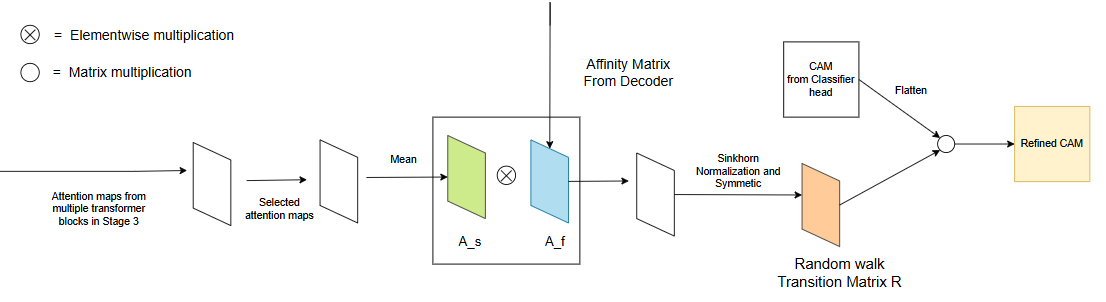
\includegraphics[width=0.9\textwidth]{refinement.png}}
    \caption{CAM refinement by exploiting affinity map}
    \label{fig:refinement}
\end{figure}

\subsection{Random Walk Propagation}
\label{subsec:random_walk}

The refined class activation map (CAM) for a specific class $c$, denoted as $M^c_f$ is found by random walk propagation as follows:

\begin{equation}
    M_f^c = B^c \odot T^\alpha \cdot M_{\text{init}}^c
\end{equation}

where, $M^c_{\text{init}} \in \mathbb{R}^{hw \times 1}$ is the initial CAM for class $c$, reshaped into vector form. $T$ is the transition probability matrix, $\alpha$ is the hyperparameter that controls the strength of the refinement we want to apply. It is equivalent to the number of iterations of the random walk propagation. \( B^c \in \mathbb{R}^{1 \times hw} \) is the box mask obtained from the CAM of class \( c \), and \( \odot \) denotes the Hadamard product. This masking is needed to restrict the refining region spatially. It is obtained for each target class c by thresholding the CAM of this class by a constant. The connected regions of the mask map are found and covered by minimum rectangle bounding boxes. These boxes mask the affinity of distant pixels, preventing over-expansion.

Finally, the refined CAM $M^c_f$ is passed through an online post-processing module - specifically, the pixel-adaptive refinement module proposed in \cite{wsss_afa_affinity_from_attention}.

\subsection{Pixel Adaptive refinement module}
\label{subsec:par}
To ensure local consistency, pixel-adaptive convolution is introduced by \cite{wsss_afa_affinity_from_attention}. It uses local RGB and spatial information to define the low-level pair-wise semantic affinity of two pixels. Given an input image \( I \in \mathbb{R}^{h \times w \times 3} \), the pairwise affinities between two pixels at positions \((i, j)\) and \((k, l)\) is calculated as follows:

- \( \kappa^{\text{rgb}}_{ij,kl} \) measures color similarity (the closer the colors, the higher the affinity).

- \( \kappa^{\text{pos}}_{ij,kl} \) measures spatial closeness (pixels closer in space have higher affinity).

These are defined as:

\[
    \kappa^{\text{rgb}}_{ij,kl} = -\frac{\| I_{ij} - I_{kl} \|^2}{w_1 \sigma^2_{\text{rgb}}}, \quad
    \kappa^{\text{pos}}_{ij,kl} = -\frac{\| P_{ij} - P_{kl} \|^2}{w_2 \sigma^2_{\text{pos}}}
\]

Here:
- \( I_{ij} \) and \( P_{ij} \) are the RGB values and 2D spatial coordinates at pixel \((i, j)\),
- \( \sigma_{\text{rgb}} \) and \( \sigma_{\text{pos}} \) are the standard deviations of color and position differences,
- \( w_1 \) and \( w_2 \) are weights that control smoothness.

Then, the affinity kernel \( \kappa_{ij,kl} \) for each pixel pair is computed by applying a softmax to normalize both terms across the local neighborhood \( \mathcal{N}(i, j) \), and combining them:

\[
    \kappa_{ij,kl} = \frac{ \exp(\kappa^{\text{rgb}}_{ij,kl}) }{ \sum\limits_{(x, y) \in \mathcal{N}(i, j)} \exp(\kappa^{\text{rgb}}_{ij,xy}) }
    + w_3 \cdot \frac{ \exp(\kappa^{\text{pos}}_{ij,kl}) }{ \sum\limits_{(x, y) \in \mathcal{N}(i, j)} \exp(\kappa^{\text{pos}}_{ij,xy}) }
\]

Here, \( w_3 \) is a weight to balance the influence of the position term.

This affinity kernel is used to iteratively refine a CAM \( M \in \mathbb{R}^{h \times w \times C} \). At iteration \( t \), each pixel value \( M^t_{i,j,c} \) for class \( c \) is updated by aggregating class scores from neighboring pixels weighted by the affinity:

\begin{equation}
    M^t_{i,j,c} = \sum_{(k, l) \in \mathcal{N}(i, j)} \kappa_{ij,kl} \cdot M^{t-1}_{k,l,c}
\end{equation}


The neighborhood \( \mathcal{N}(i, j) \) is defined as the 8-connected neighbors (i.e., a \(3\times{3}\) window) with multiple dilation rates  allowing the refinement to capture both local and semi-local context.

\subsection{Pseudo-Label Generation}
\label{subsec:pseudo_label_generation}
The refined CAMs are used to generate the pseudo-labels or segmentation labels, which assign a class label to each pixel (patch),
\begin{equation}
    M_p(x, y) = \arg\max_{c \in \{1, \ldots, C\}} M_c(x, y)
\end{equation}
where \( M_c \in \mathbb{R}^{h \times w} \) is the refined CAM and \( M_p \in \mathbb{R}^{h \times w} \) is the pseudo-label.
The generated pseudo-labels are used as supervision for the segmentation network.



\section{Loss Function}
\label{subsec:loss_func}

The loss function defined by \cite{wsss_frozen_clip}:
\begin{equation}
    \mathcal{L} = \mathcal{L}_{seg} + \lambda \mathcal{L}_{aff}
\end{equation}

where, $\mathcal{L}_{aff}$ is the affinity loss and $\mathcal{L}_{seg}$ is the segmentation loss. $\lambda$ is the weighting parameter.
\subsection{Affinity Loss}
\label{aff_loss}

In the refinement module, we used the affinity map of the decoder features, $A_f$ (\autoref{eq: A_f}). The quality of the final pseudolabel directly depends on it. We need to ensure that the pairwise affinity of the pseudolabel matches the pairwise affinity of the decoder output, because that is what the random walk propagation implies.
We compute the affinity labels for the predicted pseudolabel as follows:

\begin{equation}
    \hat{A} = O_h(M_p)^TO_h(M_p)
\end{equation}
where $O_h(.)$ is the one-hot encoding of $M_p$, and $A \in \mathbb{R}^{hw \times hw}$  is the affinity label.
. This means that the value of $\hat{A(i,j)}$ will be 1 for the $(i,j)$ pair which have the same class label, and 0 otherwise. The affinity loss is the Cross-Entropy Loss of $A_f$ and $\hat{A}$:
\begin{equation}
    \mathcal{L}_{aff} = \mathcal{L}_{ce}(A_f, \hat{A})
\end{equation}

\subsection{Segmentation Loss}
\label{seg_loss}
We obtain the segmentation prediction, $P$, from the decoder (\autoref{eq:prediction}). As we are using the refined CAM or pseudolabel, $M_p$ as supervision, the segmentation loss is computed:

\begin{equation}
    \mathcal{L}_{seg} = \mathcal{L}_{ce}(P, M_p \uparrow)
\end{equation}

where \( L_{ce} \) is the cross-entropy loss, and \( M_p{\uparrow} \in \mathbb{R}^{H \times W} \). $H$ and $W$ are the original height and width of the image respectively.


